% https://github.com/xinychen/awesome-latex-drawing
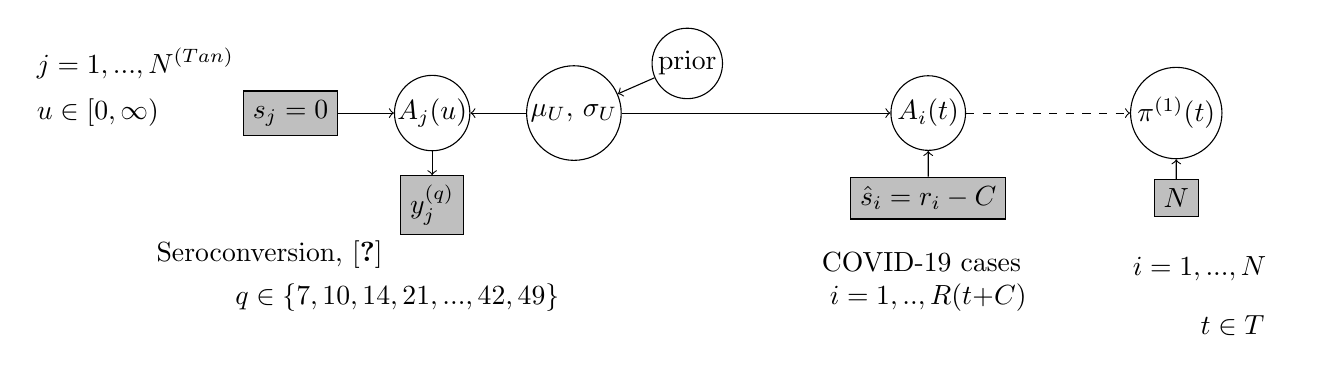
\begin{tikzpicture}[scale=0.9]
    
    % Tan model
    
    % N
    \node [text width=5cm] (TanN) at (-2.8, 2.7)  {$j = 1, ..., N^{(Tan)}$};    
    
    % d
    \node [text width=5cm] (Ttan) at (-2.8, 2)   {$u  \in [0, \infty)$};

    % S
    \node [rectangle,draw=black,fill=lightgray] (S) at (-2, 2) {$s_j = 0$};  
    
    % A
    \node [circle,draw=black,fill=white,inner sep=0pt,minimum size=0.6cm] (Atan) at (0, 2) {$A_j(u)$};
    
    % mu U , sigma U
    \node [circle,draw=black,fill=white,inner sep=1pt,minimum size=0.5cm] (musigma) at (2, 2) {$\mu_U$, $\sigma_U$};
  
    % prior 
    \node [circle,draw=black,fill=white,inner sep=1pt,minimum size=0.5cm] (musigmaprior) at (3.6, 2.7) {prior};   
    
     % Seroconversion
    
    % y
    \node [rectangle,draw=black,fill=lightgray] (y) at (0, 0.7) {$y_j^{(q)}$};  
    
    % label
    \node [text width=7cm] (tanlabel) at (0, 0)  {Seroconversion, \cite{Tan2020}}; 
    
    % Q
    \node [text width=5cm] (Qtan) at (0, -0.6)  {$q  \in \{7, 10, 14, 21, ..., 42, 49\}$};

    \plate[] {Y}{(y)(tanlabel)(Qtan)}{}
    
    \plate[] {TAN}{(TanN)(Y)(Atan)(musigma)(musigmaprior)}{}
    


    \path [draw,->] (Atan) edge (y);   
    \path [draw,->] (S) edge (Atan);   
    \path [draw,->] (musigma) edge (Atan); 
    
    
    % FNIDR projection
    % ---

    % projected A_i(t)
    \node [circle,draw=black,fill=white,inner sep=1pt,minimum size=0.6cm] (Ahus) at (7, 2) {$A_i(t)$};
    
    % Registered disease cases
    % ----
    
    % r_i
    \node [rectangle,draw=black,fill=lightgray] (r) at (7, 0.8) {$\hat{s}_i = r_{i} - C$}; 
    
    % label
    \node [text width=2.7cm] (obslabel) at (7, -0.1)  {COVID-19 cases}; 
    
    % i = 1, .., R(t)
    \node [text width=2.5cm] (nobs) at (7, -0.6)  {$i = 1, .., R(t + C)$}; 
    
    % plate
    \plate[] {TTR}{(r)(nobs)(obslabel)}{}   

    
    % prevalence
    \node [circle,draw=black,fill=white,inner sep=1pt,minimum size=0.6cm] (pi) at (10.5, 2) {$\pi^{(1)}(t)$};
    
    \node [rectangle,draw=black,fill=lightgray] (N) at (10.5, 0.8) {$N$}; 
    
    % HUS N
    \node [text width=2cm] (NHUS) at (11.0, -0.2)  {$i = 1, ..., N$};    

    % HUS time
    \node [text width=1cm] (T) at (11.4, -1)  {$t  \in T$};

    
    \plate[] {HUS}{(NHUS)(TTR)(Ahus)(pi)(T)}{}   
    \plate[white]{ALL}{(HUS)(TAN)}{}

    
    \path [draw,->] (musigmaprior) edge (musigma); 
        
    \path [draw,->] (musigma) edge (Ahus); 

    \path [draw,->] (r) edge (Ahus); 
    \path [draw,->, dashed] (Ahus) edge (pi); 
    \path [draw,->] (N) edge (pi); 

    
    
    
\end{tikzpicture}
